\iffalse
	\chapter{2020}
	\author{AI24BTECH11003}
	\section{xe}
\fi

%1
    \item Let $z$ be a complex number. Then the series $\underset{n=0}{\overset{\infty}{\sum}}\frac{z^{2n}}{\brak{2n}!}$ 
    \hfill{(2020)}
    

        \begin{enumerate}
            \item converges for all $z.$
            \item converges for all $\abs{z}\leq1$ and diverges for $\abs{z}>1.$
            \item converges for $z=0$ and diverges for any $z\neq0.$
            \item converges for $\abs{z}<1$ and diverges for $\abs{z}\geq1$
        \end{enumerate}


%2
    \item Let $\overrightarrow{V}\brak{x,y,z} = ax\overrightarrow{i}-bz\overrightarrow{j} +cy\overrightarrow{k}$ be a vector whose curl is zero. Then necessarily
    
    \hfill{(2020)}

        \begin{multicols}{4}
        \begin{enumerate}
            \item $a=b=c$
            \item $a=-b=c$
            \item $b=c$
            \item $b=-c$
        \end{enumerate}
    \end{multicols}

%3
    \item Let $f\brak{x}$be a continuous function on the real line such that for any x, $\int_0^{x^2}f\brak{t}dt=x^2\brak{1+x^2}$. Then $f\brak{2}$ is \rule{1cm}{0.15mm}.
    \hfill{(2020)}


%4
    \item The number of points at which the function $f\brak{x,y} = \frac{x^2}{2}+\frac{y^4}{4}-\frac{y^2}{2}$ has local minima is \rule{1cm}{0.15mm}.
    \hfill{(2020)}
    

%5
    \item Let $f\brak{t}$ be a real-valued differential function on $\brak{-1,1}$ such that $f\brak{0}=0$ and $\abs{\frac{df}{dt}}<1$ for $0<t<1$. Then the series $\underset{n=0}{\overset{\infty}{\sum}}f\brak{0.5}^n$
    \hfill{(2020)}


        \begin{enumerate}
            \item converges but not absolutely.
            \item is unbounded.
            \item converges absolutely.
            \item is bounded but does not converge.
        \end{enumerate}


%6
    \item Let $X$ be a random variable with probability density function
    
    \begin{center}
    $f\brak{t}=
    \begin{cases}
        \exp\brak{-t} & \text{for } t\geq0\\
        0 & \text{for } t<0
    \end{cases}$
    \end{center}
    
    Let $0<a<b$. Then the probability $\mathbf{P}\brak{X\leq b|X\geq a}$ depends only on
    \hfill{(2020)}

    \begin{multicols}{4}
        \begin{enumerate}
            \item $b-a.$
            \item $b.$
            \item $a.$
            \item $a+b.$
        \end{enumerate}
    \end{multicols}

%7

    \item Let $A$ be a $3\times3$ matrix such that $A^2=A$. Then it is necessary that 
    \hfill{(2020)}


        \begin{enumerate}
            \item $A$ is the identity matrix or the zero matrix.
            \item the determinant of $A^4$ is either 0 or 1.
            \item the rank of $A$ is 3.
            \item $A$ has one imaginary eigenvalue.
        \end{enumerate}


%8
    
    \item Players $A$ and $B$ take turns to throw a fair dice with six sides. If $A$ is the first player to throw, then the probability of $B$ being the first one to get a six is \rule{1cm}{0.15mm} (round off to two decimal places).
    \hfill{(2020)}

%9
        
    \item Figures below show the velocity and the shear stress profiles for the flow in a duct. In each option, '1' represents velocity profile, and '2' represents shear stress profile.

    Choose the correct option that closely represents the turbulent flow condition.
    \hfill{(2020)}

    \begin{multicols}{2}
        \begin{enumerate}
            \item \resizebox{0.625\columnwidth}{!}{
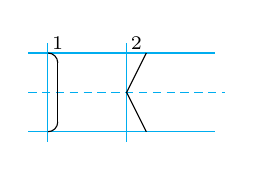
\begin{tikzpicture}
    \draw[cyan, densely dashed] (-0.25,0) to (2.25,0);
    \draw[cyan] (-0.25,0.5) to (2.125,0.5);
    \draw[cyan] (-0.25,-0.5) to (2.125,-0.5);
    \draw[cyan] (0,-0.625) to (0,0.625);
    \draw[cyan] (1,-0.625) to (1,0.625);
    \draw[black] (0,0.5) arc[start angle=90, end angle=0, radius=0.125];
    \draw[black] (0,-0.5) arc[start angle=270, end angle=360, radius=0.125];
    \draw[black] (0.125,0.375) to (0.125,-0.375);    
    \draw[black] (1.25,0.5) to (1,0) to (1.25,-0.5);
    \node at (0.125,0.625){\scriptsize 1};
    \node at (1.125,0.625){\scriptsize 2};
\end{tikzpicture}
}
            \item \resizebox{0.625\columnwidth}{!}{
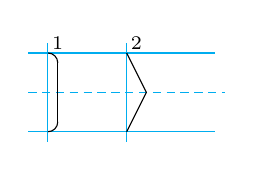
\begin{tikzpicture}
    \draw[cyan, densely dashed] (-0.25,0) to (2.25,0);
    \draw[cyan] (-0.25,0.5) to (2.125,0.5);
    \draw[cyan] (-0.25,-0.5) to (2.125,-0.5);
    \draw[cyan] (0,-0.625) to (0,0.625);
    \draw[cyan] (1,-0.625) to (1,0.625);
    \draw[black] (0,0.5) arc[start angle=90, end angle=0, radius=0.125];
    \draw[black] (0,-0.5) arc[start angle=270, end angle=360, radius=0.125];
    \draw[black] (0.125,0.375) to (0.125,-0.375);    
    \draw[black] (1,0.5) to (1.25,0) to (1,-0.5);
    \node at (0.125,0.625){\scriptsize 1};
    \node at (1.125,0.625){\scriptsize 2};
\end{tikzpicture}
}
            \item \resizebox{0.625\columnwidth}{!}{
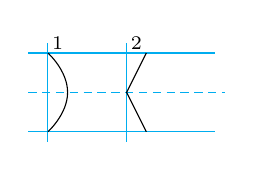
\begin{tikzpicture}
    \draw[cyan, densely dashed] (-0.25,0) to (2.25,0);
    \draw[cyan] (-0.25,0.5) to (2.125,0.5);
    \draw[cyan] (-0.25,-0.5) to (2.125,-0.5);
    \draw[cyan] (0,-0.625) to (0,0.625);
    \draw[cyan] (1,-0.625) to (1,0.625);
    \draw[black] plot [smooth, tension=1] coordinates {(0,0.5) (0.25,0) (0,-0.5)}; %1
    \draw[black] (1.25,0.5) to (1,0) to (1.25,-0.5); %2 
    \node at (0.125,0.625){\scriptsize 1};
    \node at (1.125,0.625){\scriptsize 2};
\end{tikzpicture}
}
            \item \resizebox{0.625\columnwidth}{!}{
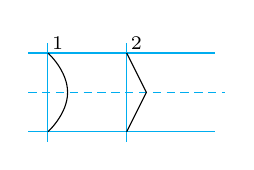
\begin{tikzpicture}
    \draw[cyan, densely dashed] (-0.25,0) to (2.25,0);
    \draw[cyan] (-0.25,0.5) to (2.125,0.5);
    \draw[cyan] (-0.25,-0.5) to (2.125,-0.5);
    \draw[cyan] (0,-0.625) to (0,0.625);
    \draw[cyan] (1,-0.625) to (1,0.625);
    \draw[black] plot [smooth, tension=1] coordinates {(0,0.5) (0.25,0) (0,-0.5)}; %1
    \draw[black] (1,0.5) to (1.25,0) to (1,-0.5); %2
    \node at (0.125,0.625){\scriptsize 1};
    \node at (1.125,0.625){\scriptsize 2};
\end{tikzpicture}
}
        \end{enumerate}
    \end{multicols}

%10
    
    \item The variation of shear stress $\brak{\tau}$ against strain rate $\brak{\frac{du}{dy}}$ is given in the Figure. Identify the line/curve among P, Q, R and S, that represents an ideal fluid.
    \hfill{(2020)}

    \begin{figure}[!ht]
\centering
\resizebox{0.3\textwidth}{!}{%
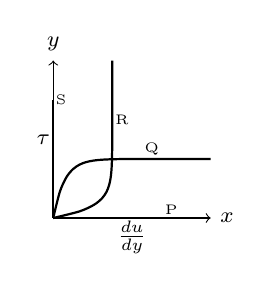
\begin{tikzpicture}
    \draw[black, ->] (0,0) to (2,0) node[right]{\footnotesize $x$};
    \node at (1,-0.25){\footnotesize $\frac{du}{dy}$};
    \draw[black, ->] (0,0) to (0,2) node[above]{\footnotesize $y$};
    \node at (-0.125,1){\footnotesize $\tau$};
    \draw[black, thick] (0,0) to (0,1.5);
    \node at (0.1,1.5){\tiny S};
    \draw[black, thick] (0,0) to (1.5,0);
    \node at (1.5,0.1){\tiny P};
    \draw[domain=0:2, smooth, variable=\x, black, thick] plot ({\x}, {0.75 - 0.75*exp(-7*\x)});
    \node at (1.25,0.875){\tiny Q};
    \draw[domain=0:2, smooth, variable=\y, black, thick] plot ({0.75 - 0.75 * exp(-7*\y)}, {\y});
    \node at (0.875,1.25){\tiny R};
\end{tikzpicture}
}%

\label{fig:my_label}
\end{figure}

    \begin{multicols}{4}
        \begin{enumerate}
            \item S
            \item P
            \item Q
            \item R
        \end{enumerate}
    \end{multicols}

%11
    
    \item A body is under stable equilibrium in a homogeneous fluid , where CG and CB are center of gravity and center of buoyancy, respectively. Two statements, '\textbf{P}' and '\textbf{Q}', are given below:\\
    \textbf{P:} For a fully submerged condition, CG should always be below CB\\
    \textbf{Q:} For a floating body, CG need not be below CB\\
    Choose the option that is valid for the present situation.
    \hfill{(2020)}


        \begin{enumerate}
            \item \textbf{P} is False, \textbf{Q} is True, when metacentre is below CG
            \item \textbf{P} is False, \textbf{Q} is True, when metacentre is above CG
            \item \textbf{P} is True, \textbf{Q} is False, when metacentre is below CG
            \item \textbf{P} is True, \textbf{Q} is False, when metacentre is above CG
        \end{enumerate}


%12
    
    \item A laminar hydrodynamic boundary layer over a smooth flat plate is shown in the Figure. The shear stress at the wall is denoted by $\tau_W$. Which one of the following conditions is correct?
    \hfill{(2020)} 

    \begin{figure}[!ht]
\centering
\resizebox{0.3\textwidth}{!}{%
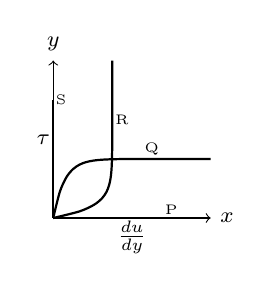
\begin{tikzpicture}
    \draw[black, ->] (0,0) to (2,0) node[right]{\footnotesize $x$};
    \node at (1,-0.25){\footnotesize $\frac{du}{dy}$};
    \draw[black, ->] (0,0) to (0,2) node[above]{\footnotesize $y$};
    \node at (-0.125,1){\footnotesize $\tau$};
    \draw[black, thick] (0,0) to (0,1.5);
    \node at (0.1,1.5){\tiny S};
    \draw[black, thick] (0,0) to (1.5,0);
    \node at (1.5,0.1){\tiny P};
    \draw[domain=0:2, smooth, variable=\x, black, thick] plot ({\x}, {0.75 - 0.75*exp(-7*\x)});
    \node at (1.25,0.875){\tiny Q};
    \draw[domain=0:2, smooth, variable=\y, black, thick] plot ({0.75 - 0.75 * exp(-7*\y)}, {\y});
    \node at (0.875,1.25){\tiny R};
\end{tikzpicture}
}%

\label{fig:my_label}
\end{figure}

    \begin{enumerate}
        \item pressure is varying along '$x$' and $\brak{\tau_w}_{x1}>\brak{\tau_w}_{x2}$
        \item pressure is constant along '$x$' and $\brak{\tau_w}_{x2}>\brak{\tau_w}_{x1}$
        \item pressure is constant along '$x$' and $\brak{\tau_w}_{x1}>\brak{\tau_w}_{x2}$
        \item pressure is varying along '$x$' and $\brak{\tau_w}_{x2}>\brak{\tau_w}_{x1}$
    \end{enumerate}



%13
    
    \item A non-dimensional number known as \textbf{Weber} number is used to characterize which one of the following flows,
    \hfill{(2020)}
    
    \begin{multicols}{2}
    \begin{enumerate}
        \item motion of fluid in open channel
        \item motion of fluid droplets
        \item motion of fluid at high velocity
        \item motion of fluid through a pipe
    \end{enumerate}
    \end{multicols}
